%!TeX root=../thesis.tex
%("dica" para o editor de texto: este arquivo é parte de um documento maior)
% para saber mais: https://tex.stackexchange.com/q/78101/183146

\chapter{Reference Architecture for ML-Enabled Systems}
\label{chap:ml_enabled_systems}
%%%%%%%%%%%%%%%%%%%%%%%%%%%%%%%%%%%%%%%%%%%%%%%%%%%%%%%%%%%%%%%%%%%%%%%%%%%%%%%%

\emph{What defines an ML-enabled system?} This chapter addresses
``ML-enabled systems'' from a software architecture perspective,
as summarized by \cref{fig:reference_architecture}.
Its typical components are explored in detail in
\crefrange{sec:ref_data_acquisition}{sec:ref_monitoring}.
% Connecting with example
Afterward, \cref{chap:the_spira_system} provides a real-world practical
example of an ML-enabld system, designed by the authors in the early days
of this PhD research~\parencite{Ferreira2022SPIRA:Detection}.
% Connecting with goals
Understanding the general architecture of ML-enabled systems will delimit
the scope of the research questions, introduced in \cref{chap:introduction}.
Moreover, it will support the methodology proposed to answer them,
detailed in \cref{chap:research_methodology}.

% First, \cref{sec:reference_architecture} explores a reference
% architecture for these systems, describing their typical components.
% Then, \cref{sec:example_spira_system} provides a real-world practical example
% of an ML-enabled system, designed by the authors in the early days of this
% PhD research~\parencite{Ferreira2022SPIRA:Detection}.

% Understanding the boundaries of ML-enabled systems will limit the scope
% of the research questions listed in \cref{sec:research_questions}.
% and introduce concepts that will be necessary to answer them
% \cref{chap:research_methodology}.

% The basic idea of MLES: it contains a ML model
% 
% - ML models have a big lifecycle to be produced (CRISP-DM / TDSP)
% - Most of the _modelling_ is an (adhoc) experimental process to create a PoC
% - If the problem _can be solved_ with ML... then building a MLES is a problem! (yay)
% - Why a single model is not enough? Drift happens, retraining has to happen...
%   We actually need a *factory of models*
% - Sculley (and others) identified a big problem in most of this training code
%   (later confirmed by others): it is amateur, bad quality, pipeline jungles
% - Actually, the ML model is just a small piece of the whole (Sculley introduced
%   this idea)
% 
% - ML models have two steps in their lifecycle: training, and prediction
% - First, We need to acquire data: data pipelines...clinical exams to diagnose the illness. Patients would show up in hospitals with low levels
% - Then, we need to process the data for training, feature engineering...
% - Then, we need to be able to traing and retrain: training pipelines...
% - Finally, We need to integrate with the world: batch, streaming, APIs...
% 
% - There is no one-size-fits-all solution, we just have these general
%   "parts" of a ML-enabled system: data acquisition, training, prediction
% 
% - Where do we want to understand how metrics help: 
%   - Compare different types of serving?
%   - Compare different strategies of training?
%   - Compare different alternatives for each component?
%   - Split (or join) the execution of some pipelines?

\emph{\citetitle{Sculley2015HiddenSystems}}
by \citeauthor{Sculley2015HiddenSystems}~\parencite{Sculley2015HiddenSystems}
is considered one of the first publications about Machine Learning Engineering
(MLE)~\parencite{Serban2020AdoptionLearning}. Originally presented at
\mbox{NeurIPS 2014}, it has influenced the field by raising an important
consideration: \emph{Machine Learning (ML) models are only a small part
of real-world ML-enabled systems}~\parencite{Sculley2015HiddenSystems}.
In summary, the authors acknowledge that production ML-enabled systems
need many traditional software-based components to support the lifecycle
of an ML model. Henceforth, this section builds upon this understanding.

%----------------------------------------------------------------------------%
\begin{figure}[p]
  \centering
  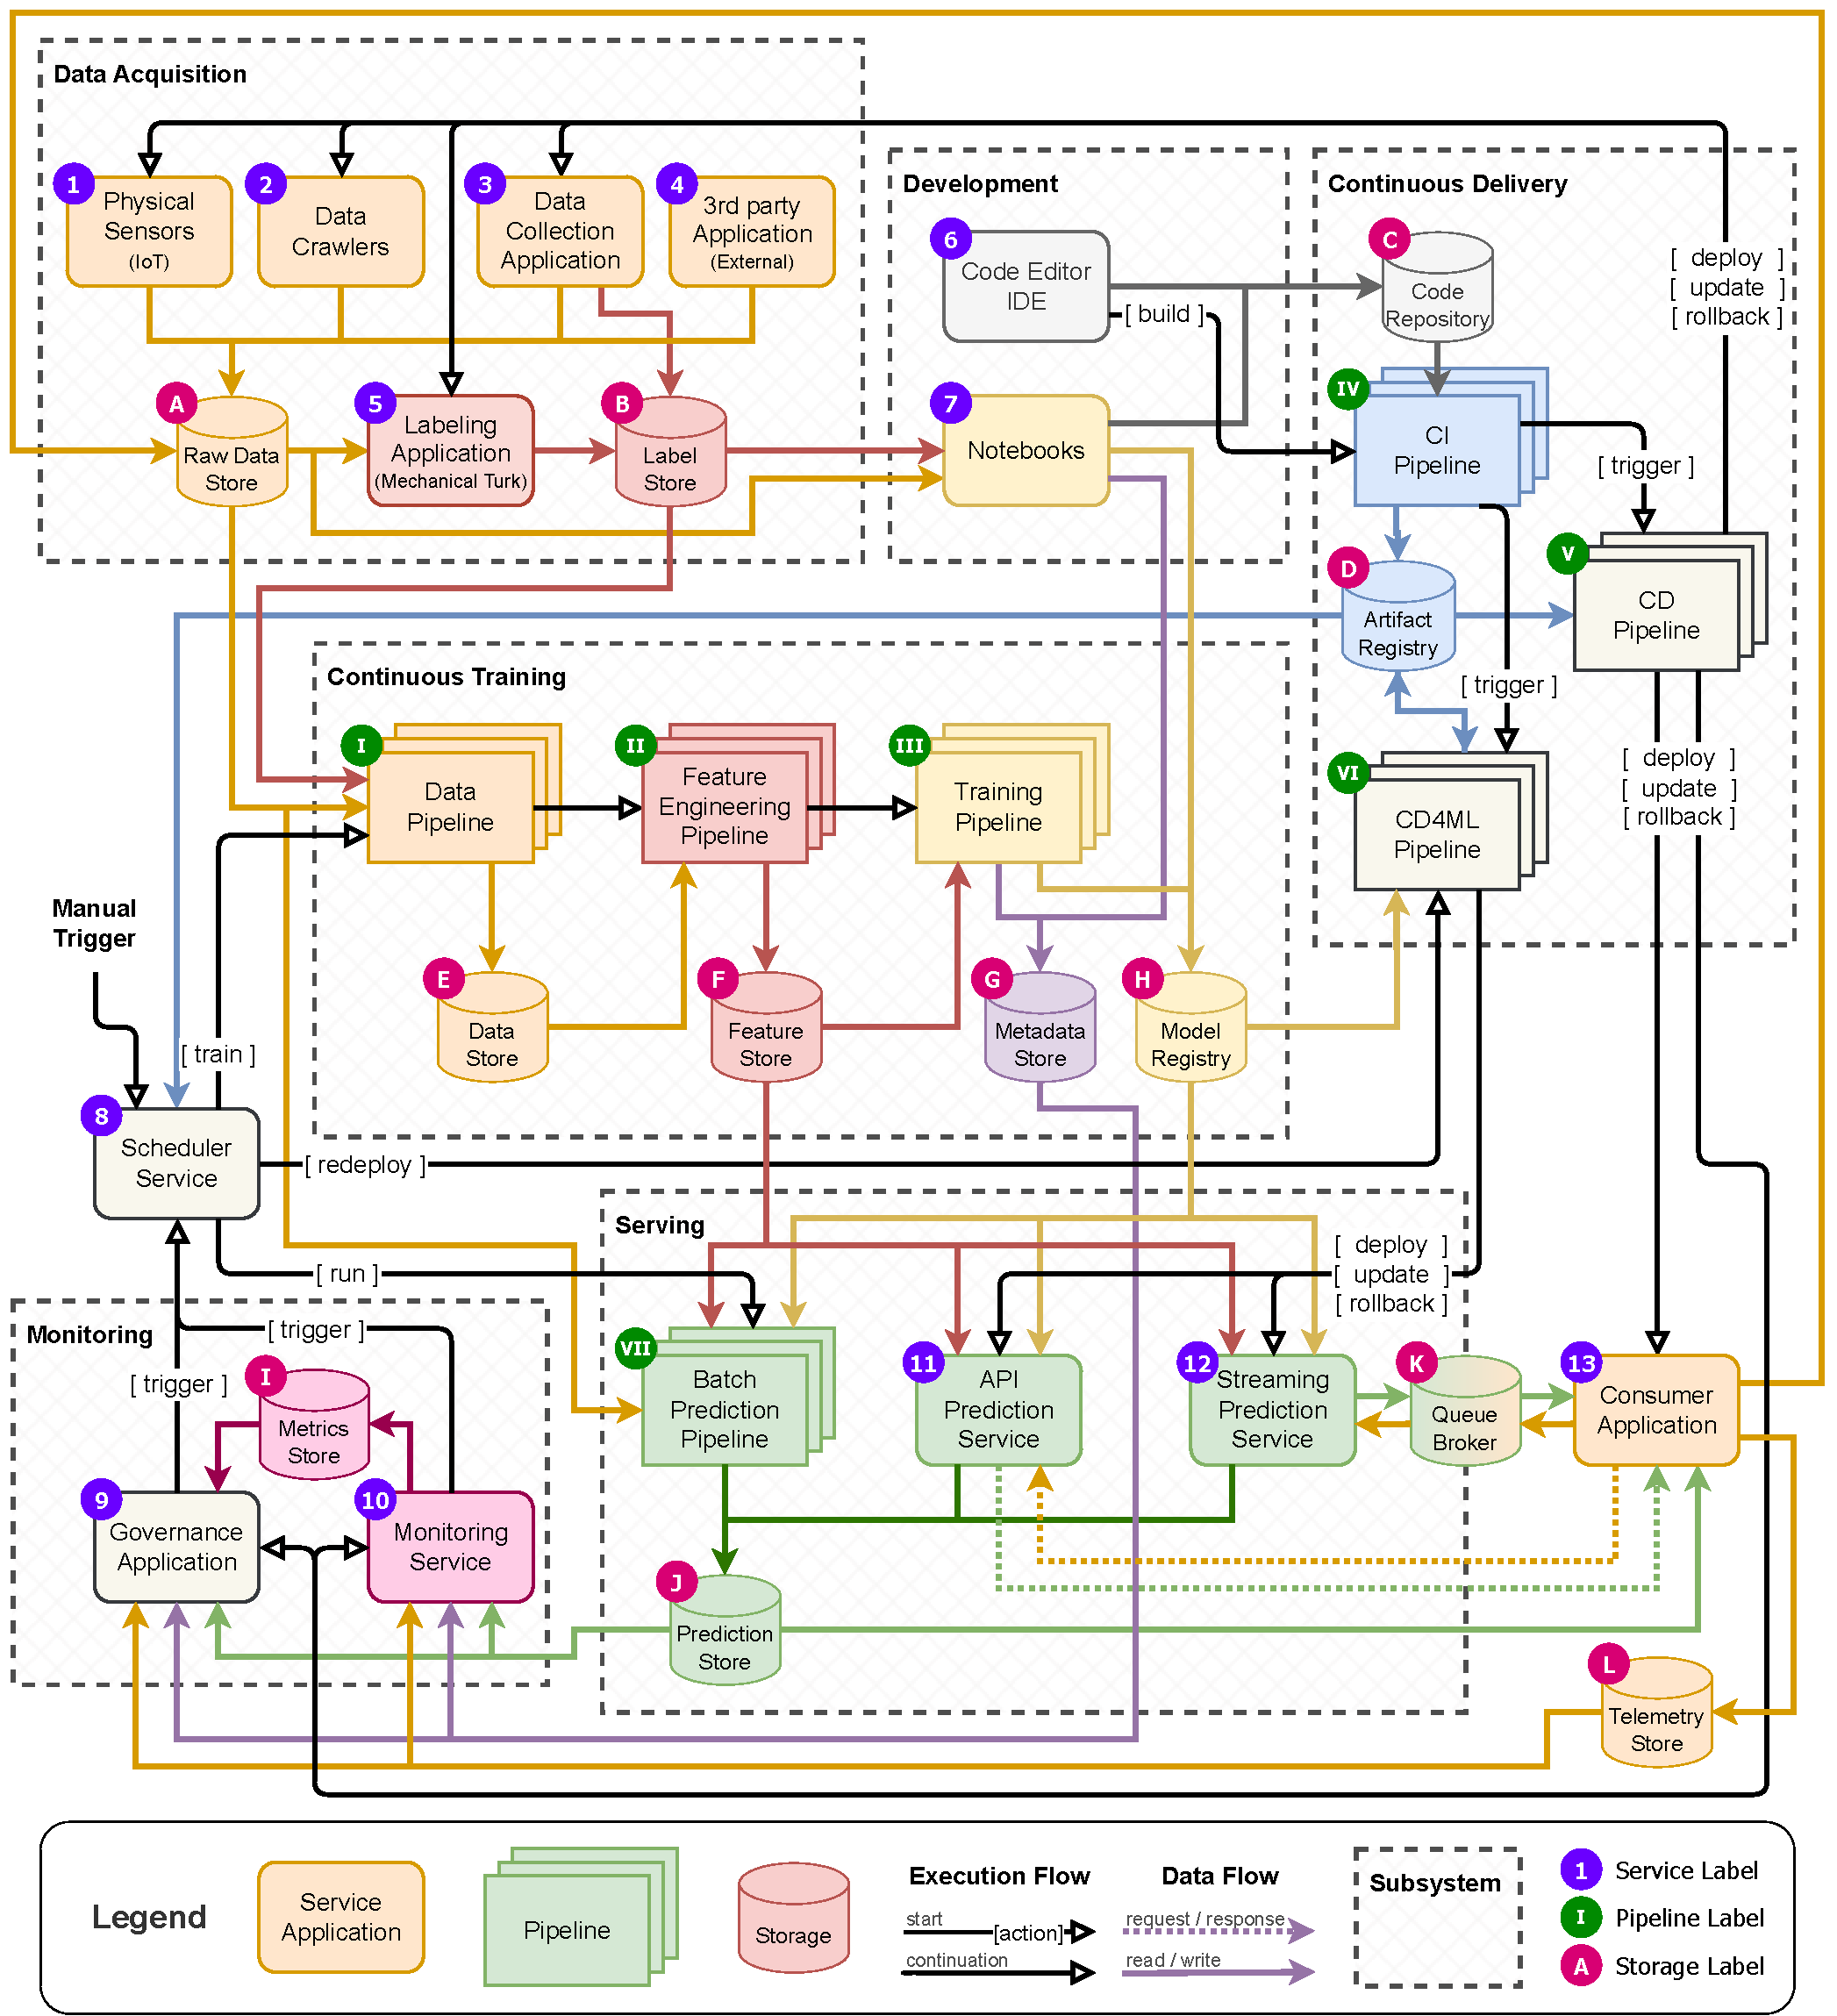
\includegraphics[width=\linewidth]{figures/Architecture.pdf}
  \caption[%
    Reference Architecture for ML-enabled Systems
  ]{%
    \emph{Reference Architecture for ML-enabled Systems.}
    There are three types of components in an ML-enabled system.
    Rectangles represent \textbf{applications} or \textbf{services},
      which execute continuously.
    Stacked rectangles represent \textbf{pipelines},
      which execute a task on demand.
    Lastly, cylinders represent \textbf{data storage},
      which may be databases of any type.
    Components are connected by arrows.
    Black arrows with a hollow tip illustrate the \textbf{execution flow}.
      They start and end in a component.
      Labeled arrows represent the trigger that starts a workflow,
      whereas unlabeled arrows represent the continuation of an
      existing workflow.
    Colored arrows with a filled tip illustrate the \textbf{data flow}.
    They appear in two types:
      solid arrows going to and from a data storage represent
      write and read operations, respectively;
      dotted arrows represent a sync or async request-response
      communication between components.
    Components are colored according to the data they produce:
      \mbox{\LegendColoredComponent{orange}{raw data}},
      \mbox{\LegendColoredComponent{red}{ML-specific data}},
      \mbox{\LegendColoredComponent{gray}{source code}},
      \mbox{\LegendColoredComponent{blue}{executable artifacts}},
      \mbox{\LegendColoredComponent{yellow}{ML models}},
      \mbox{\LegendColoredComponent{purple}{ML training metadata}},
      \mbox{\LegendColoredComponent{green}{ML model predictions}}, and
      \mbox{\LegendColoredComponent{pink}{ML model metrics}}.
      Remaining \LegendBWComponent{standalone components} orchestrate
      the execution of others.
    Components are also grouped into \textbf{subsystems}.
    % that handle all major tasks of an ML-enabled system.
    \LegendColoredLabel{violet}{Numbers},
    \LegendColoredLabel{moss}{roman numerals} and
    \LegendColoredLabel{magenta}{letters}
    are used as labels throughout \cref{chap:ml_enabled_systems}.
  }
  \label{fig:reference_architecture}
\end{figure}
%----------------------------------------------------------------------------%

\Cref{fig:reference_architecture} presents a reference architecture for ML-enabled
systems. It is based on the study by \citeauthor{Kumara2023ArchitectingPractice}%
~\parencite{Kumara2023ArchitectingPractice},
  who proposed it using Grounded Theory%
  ~\parencite{Wohlin2012ExperimentationEngineering}
  on data collected via a Multivocal Literature Review%
  ~\parencite{Garousi2019GuidelinesEngineering}.
\Cref{fig:reference_architecture} summarizes possible components of
an ML-enabled system, including
  \emph{applications and services}~\parencite{
    Newman2015BuildingMicroservices, % Microservices
    Richardson2018MicroservicesPatterns, % Microservices & monoliths
  },
  \emph{pipelines}~\parencite{
    Humble2010ContinuousAutomation, % CI/CD pipelines
    Huyen2022DesigningApplications, % ML pipelines
    Richards2020FundamentalsApproach, % Data pipelines
    Sato2019ContinuousLearning, % CD4ML pipelines
  }, and
  \emph{data storage}~\parencite{
    Kleppmann2017DesigningSystems, % Streaming
    Lakshmanan2020MachineMLOps, % Model Registry, Feature Store, etc.
    Reis2022FundamentalsSystems, % Data Engineering in general
    Sadalage2012NoSQLPersistence, % NoSQL databases
  }.
Moreover, it shows how they interact according to the system's
\emph{execution flow} and \emph{data flow}.

As illustrated in \cref{fig:reference_architecture}, the reference
architecture groups all components into six \emph{subsystems}, which
represent the major tasks of an ML-enabled system. They are:
%----------------------------------------------------------------------------%
\begin{enumerate}
  \item \nameref{sec:ref_data_acquisition}: \\
        Components that collect data from outside the system.
  \item \nameref{sec:ref_development}: \\
        Components that support experimentation and evolution of the system.
  \item \nameref{sec:ref_continuous_delivery}: \\
        Components that build and deploy the system for execution.
  \item \nameref{sec:ref_continuous_training}: \\
        Components that produce machine learning models.
  \item \nameref{sec:ref_serving}: \\
        Components that make machine learning models available for use.
  \item \nameref{sec:ref_monitoring}: \\
        Components that track the execution of machine learning models.
\end{enumerate}
%----------------------------------------------------------------------------%

\Cref{fig:reference_architecture} differs from the results presented
by \citeauthor{Kumara2023ArchitectingPractice}%
~\parencite{Kumara2023ArchitectingPractice} because it proposes
two additional subsystems:
  \nameref{sec:ref_data_acquisition},
  illustrating components that were not explicitly addressed
  in their reference architecture; and
  \nameref{sec:ref_continuous_delivery},
  associating some components that were not grouped in
  their reference architecture.

  \section{Data Acquisition}
  \label{sec:ref_data_acquisition}
  %%%%%%%%%%%%%%%%%%%%%%%%%%%%%%%%%%%%%%%%%%%%%%%%%%%%%%%%%%%%%%%%%%%%%%%%%%%%

  According to \citeauthor{Abu-Mostafa2012LearningData},
  \emph{Machine Learning} (ML) is the idea of \emph{learning from data},
  i.e., developing a data-based empirical solution when an analytical
  solution is not available~\parencite{Abu-Mostafa2012LearningData}.
  The process of learning is known as \emph{training}. It results in
  a data-based \emph{model}, whose \emph{parameters} are estimated from
  example data. Learning algorithms can be categorized into different
  types~\parencite{RussellS2021Artificial4th}, useful for specific problems,
  including:
  %--------------------------------------------------------------------------%
  \begin{itemize}
      \item \emph{supervised learning}, for classification, regression,
            and ranking;
      \item \emph{unsupervised learning}, for clustering and anomaly
            detection; and
      \item \emph{reinforcement learning}, for finding the best policy
            to choose between actions.
  \end{itemize}
  %--------------------------------------------------------------------------%
  The training dataset works a \emph{ground truth} for the ML model%
  ~\parencite{Burkov2020MachineEngineering}. For supervised learning,
  data also requires \emph{labels}, i.e., results the model should learn
  to predict~\parencite{RussellS2021Artificial4th}.

  The \nameref{sec:ref_data_acquisition} subsystem involves components that
  gather \emph{raw data} into a \LegendDataStore{A}{raw data store} for an
  ML-enabled system. There are five major sources:
  %--------------------------------------------------------------------------%
  \begin{enumerate}
    \item \LegendService{1}{physical sensors (IoT)},
          that capture data from the real world;
    \item \LegendService{2}{data crawlers},
          that scrap data from publicly available sources;
    \item \LegendService{3}{data collection applications},
          that provide specialized means to input data;
    \item \LegendService{4}{3rd party providers},
          that sell data as a product; and
    \item \LegendService{13}{consumer applications},
          that capture data influenced by model predictions.
          % that capture data -- implicitly or
          % explicitly -- that can be used later to improve the model.
  \end{enumerate}
  %--------------------------------------------------------------------------%

  An ML-enabled system can contain many data sources of multiple types.
  Each type of data source provides its own integration challenges.
  In particular, if an ML-enabled system uses data from
  \LegendService{13}{consumer applications}, it is also an
  \emph{Intelligent System}~\parencite{Hulten2018BuildingEngineering},
  i.e., a system that uses machine learning to influence itself.
  This creates \emph{feedback loops}, which are a known source of
  complexity in ML-enabled systems%
  ~\parencite{Menshawy2024NavigatingDeployment,Sculley2015HiddenSystems}.

  For ML-enabled systems that use supervised learning, there is one extra
  challenge: \emph{labeling data}.
  % Problems with labels
  Fortunately, some systems may produce labels by themselves,
  saving them in a \LegendDataStore{B}{label store}.
  % Example: recommender systems
  For example, a recommender system: after showing products to
  clients, it can use visualizations, clicks, and purchases as a proxy
  to determine the best recommendation~\parencite{Bernardi2019150Booking.com}.
  % Problems without labels
  Unfortunately, other problems have no intrinsic way to automate labeling.
  % Example: image classification
  For example, a social network system: there is no way to automatically identify
  whose faces are in a photo, unless a human starts tagging their friends first%
  ~\parencite{Tufail2023AdvancementsAlgorithms}.
  % We need mechanical turk
  For these scenarios, a separate \LegendService{5}{labeling application} or an
  integrated workflow may be used to generate labels.
  Otherwise, this process can be outsourced to a 3rd party service known as a
  \LegendService{5}{Mechanical Turk}\mbox{~\parencite{Buhrmester2018AnUse,
  SambasivanShivaniKapaniaHannahHighfll2021EveryoneAI}}.
  % And we have data augmentation, because life is hard...
  Regardless, when labels are difficult to obtain -- due to cost, ethical
  limitations, etc. -- some systems can also rely on \emph{automated labeling}
  techniques~\parencite{Ratner2017Snorkel}, such as the ones used for
  \emph{weakly} or \emph{semi-supervised learning}%
  ~\parencite{RussellS2021Artificial4th}.

  The raw data and labels collected by the \nameref{sec:ref_data_acquisition} 
  components are used both by the \nameref{sec:ref_development} and the
  \nameref{sec:ref_continuous_training} components.

  \section{Development}
  \label{sec:ref_development}
  %%%%%%%%%%%%%%%%%%%%%%%%%%%%%%%%%%%%%%%%%%%%%%%%%%%%%%%%%%%%%%%%%%%%%%%%%%%%

  The task of applying a Machine Learning (ML) model to solve a problem
  is called \emph{modelling}~\parencite{Abu-Mostafa2012LearningData}.
  This task is usually carried out by \emph{Data Scientists}%
  ~\parencite{Kim2018DataChallenges,Nahar2021MoreProjects,
  Wilson2022MachineAction}, a role that specializes in knowledge about
  ML algorithms and techniques. However, modelling starts before coding,
  with steps like \emph{business understanding} and \emph{data exploration}%
  ~\parencite{Microsoft2021TeamDocumentation,Shearer2000TheMining}.
  Two business processes became popular to describe this workflow%
  ~\parencite{Banerjee2017TwoHub,DeSilva2022AnProduction,
  Watanabe2019PreliminaryProcess}, namely:
  %--------------------------------------------------------------------------%
  \begin{itemize}
    \item the Cross-Industry Standard Process for Data Mining (CRISP-DM)%
          ~\parencite{Shearer2000TheMining,Wirth2000CRISP-DMMining}, and
    \item the Team Data Science Process (TDSP)%
          ~\parencite{Microsoft2021TeamDocumentation,Tab2017WhatDocs}.
  \end{itemize}
  %--------------------------------------------------------------------------%

  Created in the early 2000s, CRISP-DM describes best practices for data
  mining, but its simplicity made it a popular, viable description for the
  data science workflow~\parencite{Martinez-Plumed2021CRISP-DMTrajectories}. 
  Similarly, Microsoft documented TDSP from the company's experience building
  data products for different domains, focusing on a modern understanding of
  data science~\parencite{Microsoft2021TeamDocumentation}.

  The most popular tool for modelling are \LegendService{7}{notebooks},
  in particular, \href{https://jupyter.org/}{Jupyter Notebooks}. They allow
  a mix of code and documentation that follows the literate programming style%
  ~\parencite{Pimentel2019ANotebooks}. Moreover, they provide a dynamic
  environment for experimentation: by keeping the execution state in-memory,
  data scientists can quickly test different models, hyperparameters,
  training algorithms, etc.
  
  To keep track of experiments, data scientists can save their trained
  ML models in a \LegendDataStore{H}{model registry} and export metadata
  to a \LegendDataStore{G}{metadata store}%
  ~\parencite{Kreuzberger2023MachineArchitecture,Symeonidis2022MLOpsChallenges, 
  Wazir2023MLOps:Review}. There are specialized open-source and commercial tools
  that can make both these roles, such as \href{https://mlflow.org}{MLFlow} or
  \href{https://neptune.ai}{Neptune.ai}~\parencite{Kreuzberger2023MachineArchitecture}.
  However, according to \citeauthor{Lakshmanan2020MachineMLOps}, this usage
  can also be considered a type of \emph{machine learning design pattern}%
  ~\parencite{Lakshmanan2020MachineMLOps}.

  Unfortunately, using \LegendService{7}{notebooks} often leads to poor
  coding practices~\parencite{Ferreira2024BeingProject,Pimentel2019ANotebooks,
  Shankar2022OperationalizingStudy}, which makes them unsuitable for
  long-term maintainability. As a consequence, once a \emph{proof of concept}
  is validated -- by choosing the ML model, data processing, etc. --
  the code in \LegendService{7}{notebooks} can be rewritten%
  ~\parencite{Ferreira2024BeingProject,Huyen2022DesigningApplications,
  Wilson2022MachineAction}. This code becomes the backbone of the production
  ML-enabled system, as part of multiple pipelines discussed later:
    \LegendPipeline{I}{data processing},
    \LegendPipeline{II}{feature engineering}, and
    \LegendPipeline{III}{model training}.
  % the \nameref{sec:ref_continuous_training} subsystem.
  
  The production version of an ML-enabled system is built following standard
  software engineering practices~\parencite{Huyen2022DesigningApplications, 
  Wilson2022MachineAction}. Therefore, it is developed with the same tools
  used for other systems: \LegendService{6}{code editors} or 
  \LegendService{6}{Integrated Development Environments (IDEs)}.
  Moreover, all source code created can be versioned with
  popular tools like \href{https://git-scm.com}{Git},
  and stored in an online \LegendDataStore{C}{code repository} like
  \href{https://github.com}{GitHub} or \href{https://gitlab.com}{GitLab}.
  \LegendService{7}{Notebooks} are also versioned the same way,
  but support for them is much more primitive.
  In particular, \href{https://git-scm.com}{Git}-based tools lack
  native features to compare versions or annotate code reviews in
  \LegendService{7}{notebooks}~\parencite{Ferreira2024BeingProject}.

  The source code produced by the \nameref{sec:ref_development} tools is
  used by the \nameref{sec:ref_continuous_delivery} components for building
  and deploying the ML-enabled system. Pushing a new version of production
  source code to the \LegendDataStore{C}{code repository} should trigger
  this process. The ML metadata -- in particular, training metrics --
  in the \LegendDataStore{D}{metadata store} are accessed by the 
  \nameref{sec:ref_monitoring} components to track the performance
  of the ML-enabled system.

  \section{Continuous Delivery}
  \label{sec:ref_continuous_delivery}
  %%%%%%%%%%%%%%%%%%%%%%%%%%%%%%%%%%%%%%%%%%%%%%%%%%%%%%%%%%%%%%%%%%%%%%%%%%%%

  In a traditional software-based system, behavior is determined by the
  source code. A program is correct when it implements its expected behavior.
  According to~\parencite{MartinCleanCode2008}, coding is a specification
  problem~\parencite{MartinCleanArchitecture2017,MartinCleanCode2008}:
    it may be difficult to effectively translate requirements into code%
    ~\parencite{Fowler2018Refactoring:Code},
    or requirements may change through time%
    ~\parencite{Beck2001ManifestoDevelopment,Beck1999ExtremeChange}.

  In the late 1990s, the ``\citetitle{Beck2001ManifestoDevelopment}``,
  also known as the ``\emph{Agile Manifesto}'', became a symbol of
  \emph{embracing change}~\parencite{Beck2001ManifestoDevelopment}.
  The authors proposed a set of values, principles, and practices
  to enable developers to adapt to volatile requirements.
  Among the practices, they included \emph{Continuous Integration}~(CI),
  which proposes that developers working in teams should integrate their
  code into the \LegendDataStore{C}{code repository} \emph{often},
  preferably at least once a day~\parencite{Beck1999ExtremeChange}.
  This way, teams could minimize the time spent merging code,
  since the task would be split through time. Furthermore, teams
  could avoid bugs, since developers can spot errors more easily
  in less code. To verify if an integration would be successful,
  teams started creating \LegendPipeline{IV}{build and test pipelines},
  also known as \mbox{\LegendPipeline{IV}{CI pipelines}}. They first compile,
  then run a suite of automated tests against the codebase. All changes
  get double-checked in a neutral environment, usually a dedicated
  remote server. Then, any \emph{executable artifacts} produced are
  stored in an \LegendDataStore{D}{artifact registry}, which may
  be programming-language specific, or based on containers%
  ~\parencite{Kim2021TheOrganizations,Morris2020InfrastructureCode}.
  % This storage provides a single source of truth to what is running
  % in production.

  In the early 2010s, the book ``\citetitle{Humble2010ContinuousAutomation}''
  by \citeauthor{Humble2010ContinuousAutomation} proposed a
  new practice called \emph{Continuous Delivery} (CD). The authors
  expanded the CI techniques by documenting them as a design pattern%
  ~\parencite{Johnson1998ThePattern}: the \LegendPipeline{V}{deployment pipeline},
  also known as \LegendPipeline{V}{CD pipelines}. These pipelines automate
  the process of building, testing, packaging, and deploying code, thus creating
  a reliable way to get code into production. By automating the deployment,
  the authors suggested \emph{developers should always integrate their
  code in a releasable state}~\parencite{Humble2010ContinuousAutomation}.
  This requirement goes further than CI, since it also involves
  concerns about the \emph{infrastructure} where the system will be deployed%
  ~\parencite{Kim2021TheOrganizations,Morris2020InfrastructureCode}.
  In practice, CD boosts agility with a positive impact%
  ~\parencite{Forsgren2018Accelerate:Organizations}, since changes
  in a system can reach users with almost no friction.

  In 2019, the industry article \emph{\citetitle{Sato2019ContinuousLearning}}
  (CD4ML) by \citeauthor{Sato2019ContinuousLearning} presented an adaptation
  of CD for ML-enabled systems. At its core, CD4ML proposes adopting a
  \LegendPipeline{VI}{deployment pipeline}, also known as the
  \mbox{\LegendPipeline{VI}{CD4ML pipeline}}.
  % Moreover, it suggests \emph{keeping code in a releasable state}.
  % the authors listed extra challenges, since
  However, ML-enabled systems evolve via three axes of change:
  code, model, and data~\parencite{Sato2019ContinuousLearning}.
  Therefore, CD4ML requires attention to extra challenges, such as
  configuration management, data versioning, model validation, etc.%
  ~\parencite{Sato2019ContinuousLearning}. Notwithstanding, CD4ML
  fundamentally seeks enabling agility for ML-enabled systems.

  The \nameref{sec:ref_continuous_delivery} subsystem involves the three
  aforementioned pipelines. Whenever a new version of production code
  is available in the \LegendDataStore{C}{code repository},
  a \mbox{\LegendPipeline{IV}{CI pipeline}} builds, tests, and saves
  executable artifacts in the \LegendPipeline{D}{artifact store}.
  Then, it triggers a \LegendPipeline{V}{CD pipeline}, which is
  typically employed to package and deploy traditional software-based
  components. This includes any in-house services or applications from the
  \nameref{sec:ref_data_acquisition} and \nameref{sec:ref_monitoring} subsystems.
  However, for an ML-enabled component, a \LegendPipeline{VI}{CD4ML pipeline}
  needs first to package code and model, then deploy. That is the case for
  services or applications from the \nameref{sec:ref_serving} subsystem.

  Usually, \LegendPipeline{V}{CD} and \LegendPipeline{VI}{CD4ML}
  pipelines deploy a new version of a system to run into production
  infrastructure. However, if a bug is introduced, the component may
  need to go through a \emph{rollback}, where the pipeline deploys an
  older version of the component into production. To avoid outages,
  more sophisticated CD pipelines apply some deployment patterns%
  ~\parencite{Davis2019CloudPatterns}, including:
  %--------------------------------------------------------------------------%
  \begin{itemize}
    \item \emph{Blue-Green Deployments}: \\
          First, a new version of the component (\ColorBlue) is deployed.
          The older version (\ColorGreen) is still receiving all usage.
          The pipeline starts redirecting requests to the new version
          (\ColorBlue).
          If a problem is detected, requests are immediately redirected
          again to the old version (\ColorGreen).
          Otherwise, the new version (\ColorBlue) is promoted to full
          utilization.
          The old version (\ColorGreen) is kept deployed, but unused,
          for a quick rollback in case of problems discovered later.
          When a new deployment happens, the oldest version (\ColorGreen)
          is deactivated, the new version (\ColorBlue) becomes the old version,
          and a new version (\ColorGreen) is deployed.
    \item \emph{Canary Deployments}: \\
          It follows a similar process to a blue-green deployment.
          However, instead of promoting utilization immediately,
          requests are redirected in steps. This way, the system can
          be monitored for a while before the change impacts all users.
  \end{itemize}
  %--------------------------------------------------------------------------%

  Finally, since most components are \emph{stateful}, \LegendPipeline{V}{CD}
  and \LegendPipeline{VI}{CD4ML} pipelines may redeploy \emph{the same version
  of a component}, in an attempt to reset any unintended behaviors. This is
  particularly useful to solve issues with memory leak%
  ~\parencite{Davis2019CloudPatterns}.

  For services and applications, the \LegendPipeline{V}{CD} and
  \LegendPipeline{VI}{CD4ML} pipelines from the \nameref{sec:ref_continuous_delivery} 
  subsystem usually deploy components directly. However, for the pipelines
  available in the \nameref{sec:ref_continuous_training} and \nameref{sec:ref_serving}
  subsystems, there is an extra indirection: their executable artifacts are
  deployed by the \LegendService{8}{scheduler service}, which runs them
  periodically or after a manual trigger.
  The \LegendService{8}{scheduler service} may also trigger the
  \LegendPipeline{VI}{CD4ML pipeline}, after a trigger from the
  \nameref{sec:ref_monitoring} subsystem.

  \section{Continuous Training}
  \label{sec:ref_continuous_training}
  %%%%%%%%%%%%%%%%%%%%%%%%%%%%%%%%%%%%%%%%%%%%%%%%%%%%%%%%%%%%%%%%%%%%%%%%%%%%

  As described by \citeauthor{Sato2019ContinuousLearning}, ML-enabled
  systems evolve via three different axes of change: code, model, and data%
  ~\parencite{Sato2019ContinuousLearning}.
  As discussed in \cref{sec:ref_data_acquisition}, an ML model
  is the result of learning an empirical solution from data%
  ~\parencite{Abu-Mostafa2012LearningData}.
  If the learning process or the data that feeds it changes,
  then the model produced changes.

  For most ML problems, the expected behavior of a model -- its correctness --
  may \emph{change with time}~\parencite{Burkov2020MachineEngineering,
  Hulten2018BuildingEngineering}. This can happen for two reasons%
  ~\parencite{Dhinakaran2019MachineAI,Ozkaya2020WhatSystems,
  Wilson2022MachineAction}, due to:
  %--------------------------------------------------------------------------%
  \begin{itemize}
      \item a \emph{concept drift}, when the model solves a problem
            that no longer matters, i.e., the problem has changed; and
      \item a \emph{data drift}, when the model expects a data distribution
            that no longer happens, i.e., the data distribution has changed.
  \end{itemize}
  %--------------------------------------------------------------------------%

  The simplest technique to handle data drift is \emph{retraining}%
  ~\parencite{Kreuzberger2023MachineArchitecture,Lakshmanan2020MachineMLOps}:
  the same learning process is applied on new data. On the other hand,
  concept drift may require \emph{remodeling}: parameters from the learning
  process might be changed. That said, a more extreme data drift might also
  require remodeling, whereas a simpler concept drift might be solvable by
  retraining~\parencite{Wilson2022MachineAction}. Regardless, any drift
  implies generating ML models multiple times.

  The \nameref{sec:ref_continuous_training} subsystem provides
  \emph{automation} and \emph{reproducibility} for ML model generation.
  This subsystem is essential to enable \emph{Continuous Delivery
  for Machine Learning} (CD4ML)~\parencite{Sato2019ContinuousLearning}.
  As discussed in \cref{sec:ref_continuous_delivery}, the CD4ML pipeline
  packages code and model together to deploy the ML-enabled components
  from the \nameref{sec:ref_serving} subsystem. Therefore, generating a
  model needs to be a simple, reliable process%
  ~\parencite{Sato2019ContinuousLearning}.

  There are three consecutive steps for creating an ML model%
  ~\parencite{Microsoft2021TeamDocumentation,Wirth2000CRISP-DMMining},
  which originate the three pipelines in the
  \nameref{sec:ref_continuous_training} subsystem:
  %--------------------------------------------------------------------------%
  \begin{enumerate}
      \item \LegendPipeline{I}{Data Pipeline}: \\
            Raw data is cleaned, transformed, and aggregated.
            The resulting \emph{processed data} is saved in a
            \LegendDataStore{E}{data store}%
            ~\parencite{Kleppmann2017DesigningSystems,
            Reis2022FundamentalsSystems} for later use.
      \item \LegendPipeline{II}{Feature Engineering Pipeline}: \\
            Processed data is manipulated to be consumable by ML models.
            The resulting \emph{features} are saved in a
            \LegendDataStore{F}{feature store}%
            ~\parencite{Lakshmanan2020MachineMLOps} for later use.
      \item \LegendPipeline{III}{Training Pipeline}: \\
            Features and labels are consumed by a learning algorithm.
            The resulting \emph{ML model} is saved in a
            \LegendDataStore{G}{model repository}%
            ~\parencite{Lakshmanan2020MachineMLOps},
            whereas its associated \emph{ML metadata} is stored in a
            \LegendDataStore{H}{metadata repository}%
            ~\parencite{Lakshmanan2020MachineMLOps}.
  \end{enumerate}
  %--------------------------------------------------------------------------%

  All these steps are described by both data science processes
  introduced in \cref{sec:ref_development}: CRISP-DM and TDSP.
  In the \nameref{sec:ref_development} subsystem, data scientists
  do these three steps inside \LegendService{7}{notebooks} as they are 
  experimenting with a proof-of-concept. However, this code often becomes
  three separate pipelines in the \nameref{sec:ref_continuous_training}
  subsystem for a couple of reasons:
  %--------------------------------------------------------------------------%
  \begin{itemize}
    \item \emph{Big Data}: \\
          During development, a proof of concept is usually created using
          a small dataset~\parencite{Burkov2020MachineEngineering}. However,
          for training a production ML model, the amount of data may become
          a \emph{big data} problem%
          ~\parencite{Diaz-De-Arcaya2023ASurvey,Zhou2017MachineChallenges}.
          Therefore, a different stack of tools might be required to
          create a scalable, resource-efficient implementation of both
          the \LegendPipeline{I}{data pipeline} and
          the \LegendPipeline{II}{feature engineering pipeline}%
          ~\parencite{Diaz-De-Arcaya2023ASurvey,Shankar2024WeLearning}.
    \item \emph{Specialized patterns and tooling}: \\
          During development, a proof of concepts usually keeps all data
          in memory. However, this may not be viable for production.
          \emph{Feature Store} and \emph{Model Registry} are two machine
          learning design patterns~\parencite{Lakshmanan2020MachineMLOps},
          which are often implemented by specialized MLOps infrastructure
          tools~\parencite{Symeonidis2022MLOpsChallenges},
          such as \href{https://feast.dev/}{Feast} or
          \href{https://mlflow.org/}{MLFlow}.
          The same is true for \LegendDataStore{E}{data stores},
          which can be implemented via relational or non-relational
          databases~\parencite{Sadalage2012NoSQLPersistence},
          or according to different data engineering patterns%
          ~\parencite{Reis2022FundamentalsSystems},
          such as \emph{data lake} (unstructured storage),
          \emph{data warehouse} (centralized structured storage), and
          \emph{data mesh} (distributed structured storage).
          All these tools provide a natural point of separation between
          these components.
    \item \emph{Organizational Structure}: \\
          Considering Conway's Law~\parencite{Conway1968HowInvent},
          the organizational structure often reflects in the software
          architecture~\parencite{Richards2020FundamentalsApproach}.
          \LegendPipeline{I}{Data pipelines} are often built by
          \emph{data engineers}, who specialize in tools for big data
          processing~\parencite{Kleppmann2017DesigningSystems,
          Reis2022FundamentalsSystems}.
          On the other hand, implementing \LegendPipeline{II}{feature
          engineering pipelines} requires knowledge about both big data
          and machine learning tools%
          ~\parencite{Burkov2020MachineEngineering,Wilson2022MachineAction}.
          As a consequence, it might require a multidisciplinary team
          with \emph{data engineers}, \emph{data scientists},
          and \emph{machine learning engineers}%
          ~\parencite{Kim2018DataChallenges, 
          Nahar2022CollaborationProcess,Nahar2021MoreProjects}.
          Lastly, building a production \LegendPipeline{III}{training pipeline}
          requires knowledge about software engineering and machine learning%
          ~\parencite{Burkov2020MachineEngineering,Wilson2022MachineAction}.
          Therefore, it might be handled by \emph{data scientists} and
          \emph{machine learning engineers} alone%
          ~\parencite{Kim2018DataChallenges,Nahar2022CollaborationProcess,
          Nahar2021MoreProjects}.
  \end{itemize}
  %--------------------------------------------------------------------------%

  The \emph{features} in the \LegendPipeline{F}{feature store}
  and the \emph{ML models} in the \LegendPipeline{H}{model registry},
  generated by the \nameref{sec:ref_continuous_training} subsystem,
  are used by the ML-enabled components in the \nameref{sec:ref_serving} 
  subsystem. The \emph{ML metadata}, stored in the
  \LegendPipeline{G}{metadata store} after training the ML models,
  is used by the \nameref{sec:ref_monitoring} subsystem to detect
  drift, and then optionally trigger a retraining in the
  \nameref{sec:ref_continuous_training} subsystem.

  \section{Serving}
  \label{sec:ref_serving}
  %%%%%%%%%%%%%%%%%%%%%%%%%%%%%%%%%%%%%%%%%%%%%%%%%%%%%%%%%%%%%%%%%%%%%%%%%%%%

  The \nameref{sec:ref_serving} subsystem makes ML models available for use.
  After an ML model gets trained by the \nameref{sec:ref_continuous_training} 
  subsystem, it should be integrated with code that will apply the models
  into new data. These ML-enabled components are packaged by a CD4ML
  pipeline in the \nameref{sec:ref_continuous_delivery} subsystem,
  then finally deployed for usage.

  There are three major machine learning design patterns%
  ~\parencite{Lakshmanan2020MachineMLOps} to make an ML model available
  for predictions, namely:
  %--------------------------------------------------------------------------%
  \begin{enumerate}
    \item \LegendPipeline{VII}{Batch Prediction Pipeline}: \\
          A server that makes predictions in bulk after a manual
          trigger or schedule.
          Requests are received and answered via a data store.
    \item \LegendService{11}{API Prediction Service}: \\
          A server that makes predictions synchronously or asynchronously.
          Requests are received and answered via an API.
    \item \LegendService{12}{Streaming Prediction Service}: \\
          A server that makes predictions on demand.
          Requests are received and answered via
          a \LegendDataStore{K}{message broker} or
          a \LegendDataStore{K}{message queue}; and
  \end{enumerate}
  %--------------------------------------------------------------------------%
  Requests are made by a \LegendService{13}{consumer application}, which
  later may provide raw data that can be used to retrain the ML-enabled
  system, as detailed in \cref{sec:ref_data_acquisition}.

  The choice between each type of server is problem-dependent, but it can
  also be driven by the expected processing time of the ML model.
  For fast models, an \LegendService{11}{API prediction service} may be the
  simplest solution, given creating synchronous or asynchronous APIs
  is a standard practice~\parencite{Richardson2018MicroservicesPatterns}.
  However, some systems do not receive prediction requests at any time.
  In that scenario, a \LegendPipeline{VII}{batch prediction pipeline}
  might be more cost-efficient~\parencite{Kleppmann2017DesigningSystems,
  Reis2022FundamentalsSystems}. However, if processing is costly, and
  requests happen on demand, then a \LegendService{12}{streaming
  prediction service} offers the most flexible solution%
  ~\parencite{Boner2016ReactiveSystems,Smith2018MachineScale}.
  However, stream processing relies on specialized infrastructure
  tools~\parencite{Boner2016ReactiveSystems,Wampler2016FastApplications},
  in particular
    \LegendDataStore{K}{message queues}
    like \href{https://www.rabbitmq.com/}{RabbitMQ} or
    \LegendDataStore{K}{message brokers}
    like \href{https://kafka.apache.org/}{Apache Kafka}.
  % Therefore, this flexibility requires adding extra tools to the system.

  The last pattern that can be implemented alongside any of the aforementioned
  servers is the \LegendDataStore{J}{prediction store}. In its simplest form,
  it works as a cache for predictions~\parencite{Lakshmanan2020MachineMLOps,
  Sadalage2012NoSQLPersistence}. If a server receives the same request multiple
  times, and the request is costly to process, then a cache can return a
  previously calculated result, saving processing time. However, this
  solution also has important trade-offs, listed below.
  %--------------------------------------------------------------------------%
  \begin{itemize}
    \item A cache costs either memory or storage, depending on the tool
          chosen~\parencite{Sadalage2012NoSQLPersistence}. This may
          be more expensive than the cost of reprocessing requests.
    \item Some problems may process data with unbounded values.
          For example, a search system receives unstructured user textual
          input~\parencite{Manning2008IntroductionRetrieval, 
          RussellS2021Artificial4th}.
          In these scenarios, a cache can grow arbitrarily large,
          thus becoming cost-ineffective.
    \item A cache requires a careful cache invalidation strategy whenever
          a new version of the ML-enabled system is deployed. This can be
          specially tricky if the system uses any of the deployment 
          patterns discussed in \cref{sec:ref_continuous_delivery}.
  \end{itemize}
  %--------------------------------------------------------------------------%

  In its most sophisticated form, a \LegendDataStore{J}{prediction store}
  also saves a log of all predictions. This way, they may be used at a later
  stage by the  \nameref{sec:ref_monitoring} subsystem to determine if drift
  is happening, as explained in \cref{sec:ref_continuous_training}.

  \section{Monitoring}
  \label{sec:ref_monitoring}
  %%%%%%%%%%%%%%%%%%%%%%%%%%%%%%%%%%%%%%%%%%%%%%%%%%%%%%%%%%%%%%%%%%%%%%%%%%%%

  The \nameref{sec:ref_monitoring} subsystem tracks the performance of an
  ML-enabled system. As explained in \cref{sec:ref_continuous_delivery},
  \emph{concept drift} or \emph{data drift} may make an ML-enabled system
  no longer be correct. When that happens, a retrain or remodeling might
  be necessary.

  The \LegendService{10}{monitoring service} is a component that can
  automate this decision-making. This can be done in two ways:
  %--------------------------------------------------------------------------%
  \begin{itemize}
    \item \emph{Online Metrics} (at prediction time): \\
           If the ML-enabled system
           saves the historic of predictions in a 
           \LegendDataStore{J}{prediction store},
           collects its usage logs in a
           \LegendDataStore{L}{telemetry store},
           and can determine a \emph{ground truth} for its
           predictions using these data,
           then it is possible to track drift in near real-time.
    \item \emph{Offline Metrics} (at training time): \\
           If the ML-enabled system goes through periodic retraining,
           and its performance is stable, then its training performance
           metrics collected in a \LegendDataStore{G}{metadata store}
           can be used as a proxy to track drift.
  \end{itemize}
  %--------------------------------------------------------------------------%
  Between these options, the former is preferable over the latter: online
  metrics compare the model against the current behavior of users, whereas
  offline metrics depend on historic data that may no longer represent
  this current behavior.

  The \LegendService{9}{governance application} differs from the
  \LegendService{10}{monitoring service} only in its automation.
  Its goal is to cross-reference raw data, ML metadata, and predictions
  with metrics from a \LegendDataStore{I}{metrics store}. This way,
  a human decision-maker may trigger a retrain or remodeling based
  on their manual analysis.
  
  % If metrics are calculated automatically, but a human should decide,
  % then both approaches can be mixed, with metrics being exposed from the
  % \emph{monitoring service} to the \emph{governance application} via a
  % \emph{metrics store}.

  Besides drift detection, the \nameref{sec:ref_monitoring} subsystem also
  hosts another feature: AB testing~\parencite{Kohavi2020TrustworthyExperiments, 
  Lakshmanan2020MachineMLOps}. No ML model provides perfect predictions%
  ~\parencite{Burkov2020MachineEngineering,Hulten2018BuildingEngineering}.
  Therefore, it is possible to generate multiple \emph{candidate} ML models,
  all of which can be put into production \emph{at the same time}. During
  the AB test, requests are split between models, and performance metrics
  are collected for each one of them. This way, the ``best'' model
  (according to some criteria) can be promoted to full utilization.

  There are many strategies to implement AB testing%
  ~\parencite{Kohavi2020TrustworthyExperiments}. The decision between
  models may be done manually via the \LegendService{9}{governance application},
  or can be automated in the \LegendService{10}{monitoring service}.
  In the latter case, some algorithms such as \emph{Multi-Armed Bandits}
  (MAB)~\parencite{Kohavi2020TrustworthyExperiments,RussellS2021Artificial4th}
  are used by the industry to choose models automatically.

  Both the \LegendService{9}{governance application} and the
  \LegendService{10}{monitoring service} in the \nameref{sec:ref_monitoring}
  subsystem can be integrated with the \LegendService{8}{scheduler service}
  to automate the retrain or redeploy triggers. Otherwise, manual triggers
  may be done directly.
